\section{Experiments}
\label{sec:experiments}
\subsection{Kernel Ridge Regression}
\begin{figure}
\centering
\begin{tabular}{c c}
	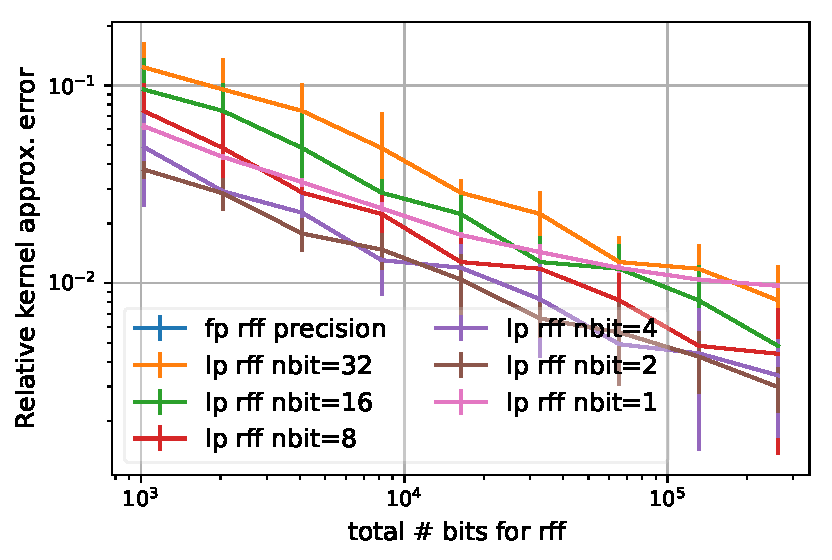
\includegraphics[width=.45\linewidth]{figures/kernel_approx_error.pdf} &
	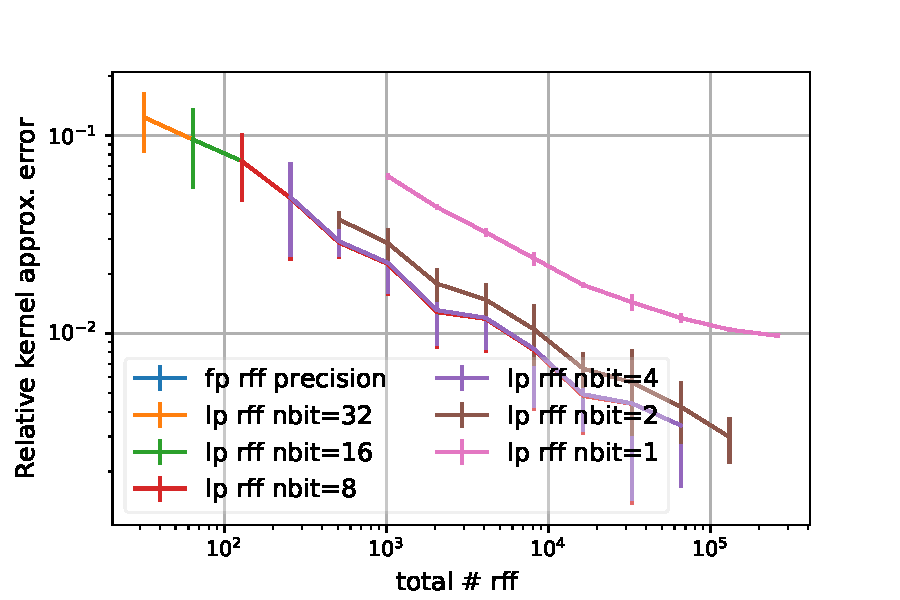
\includegraphics[width=.45\linewidth]{figures/kernel_approx_error_n_fp.pdf} \\
	(a) & (b) \\
	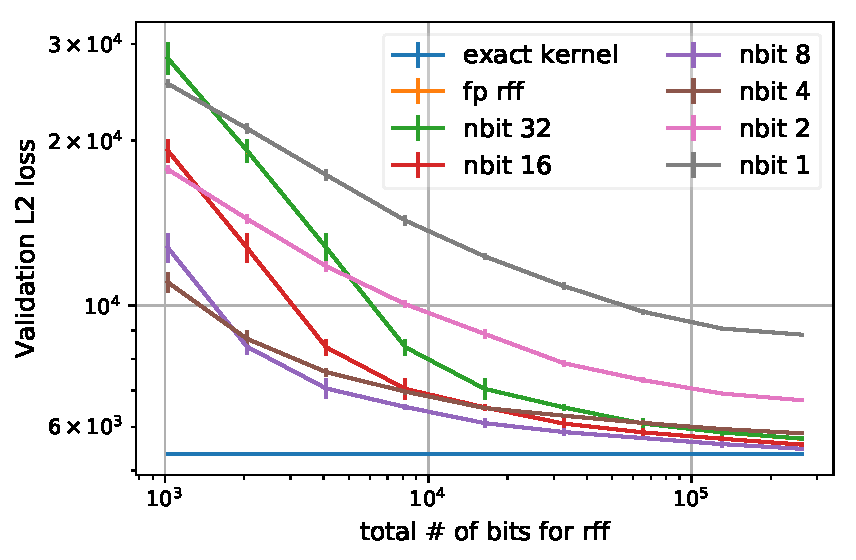
\includegraphics[width=.45\linewidth]{figures/valid_l2.pdf} &
	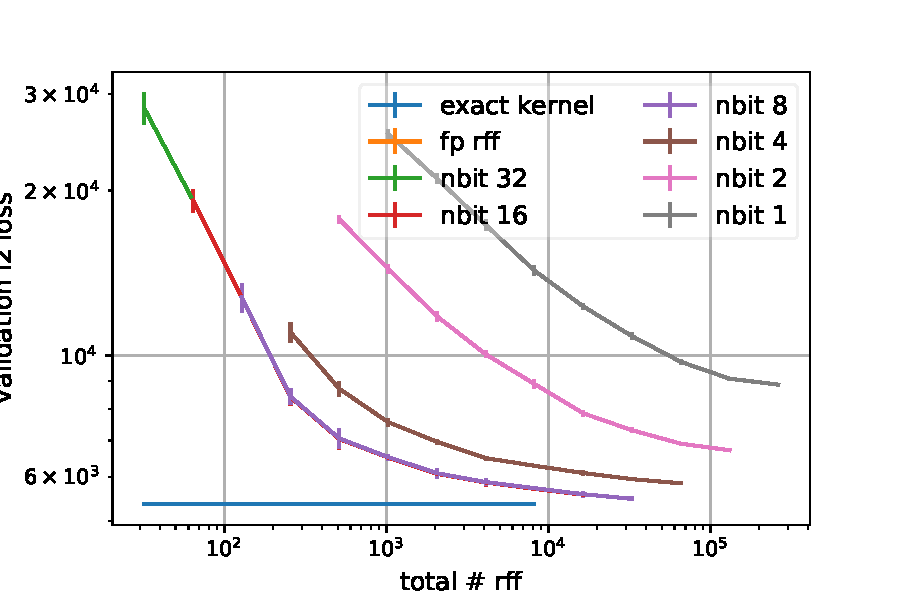
\includegraphics[width=.45\linewidth]{figures/valid_l2_n_fp.pdf}  \\
		(c) & (d) \\
\end{tabular}
\caption{Kernel approximation and validation L2 loss for Kernel Ridge Regression on UCI Census data. (a) and (b) compare different precision representation under same memory bits budgets. (c) and (d) compare different precision representation with the same number of random Fourier features.}
\label{fig:kernel_and_l2}
\end{figure}


\begin{figure}
	\centering
	\begin{tabular}{c c}
		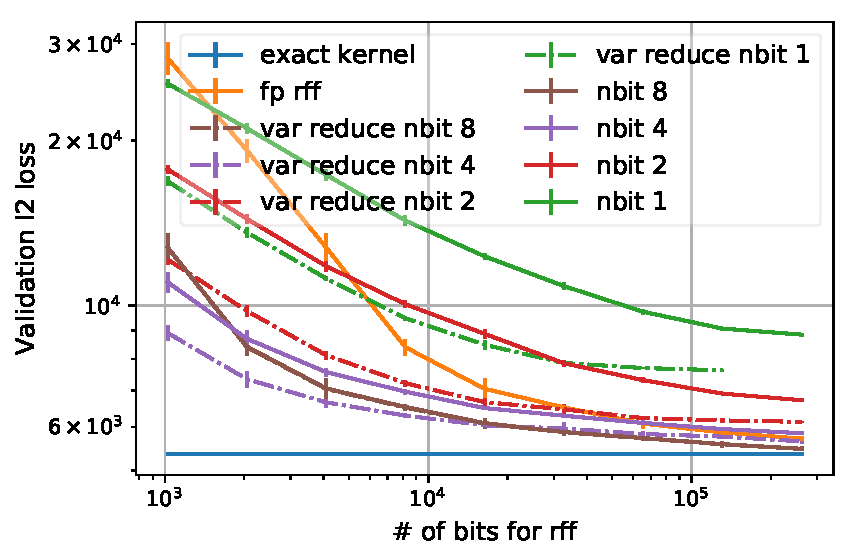
\includegraphics[width=.45\linewidth]{figures/valid_l2_var_reduction.pdf} &
		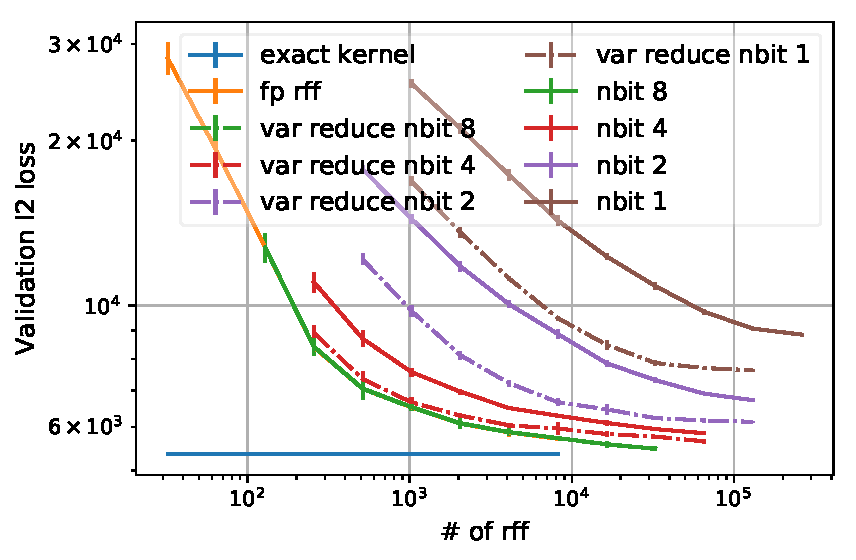
\includegraphics[width=.45\linewidth]{figures/valid_l2_n_fp_var_reduction.pdf} \\
		(a) & (b)
	\end{tabular}
	\caption{We train with low precision rffs and test with full precision rffs. Though the model is trained with low precision features, the test l2 loss can be improved by reducing variance in test rffs. (a) compare different precision representation under same memory bits budgets. (b) compare different precision representation with the same number of random Fourier features.}
	\label{fig:var_reduction}
\end{figure}


\begin{figure}
	\centering
	\begin{tabular}{c c}
%		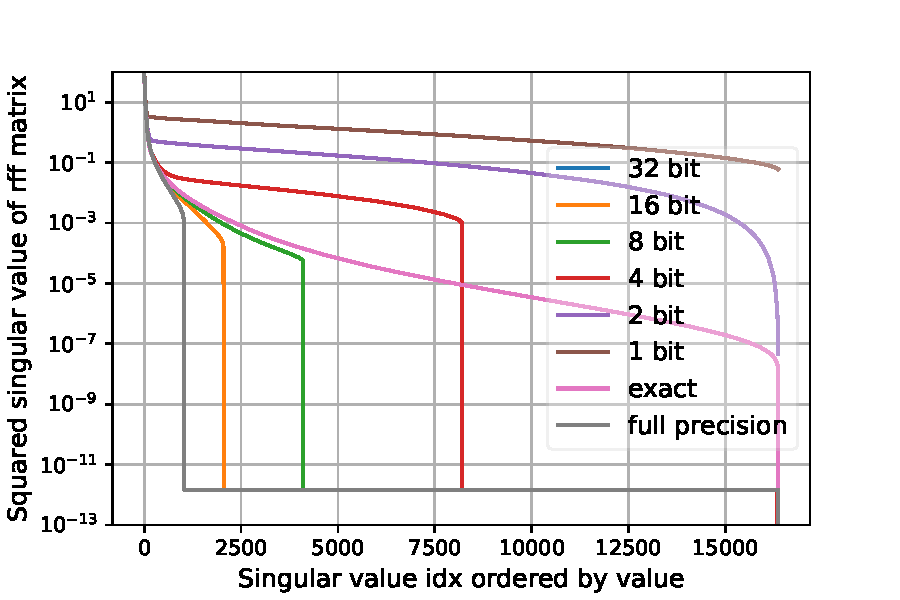
\includegraphics[width=.45\linewidth]{figures/spectrum_1024.pdf} &
		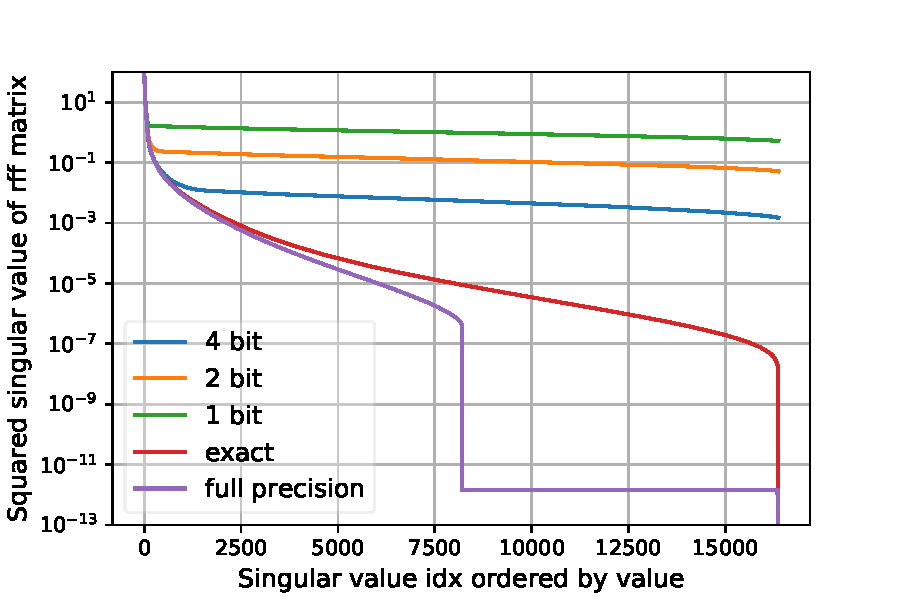
\includegraphics[width=.45\linewidth]{figures/spectrum_8192.pdf} &
		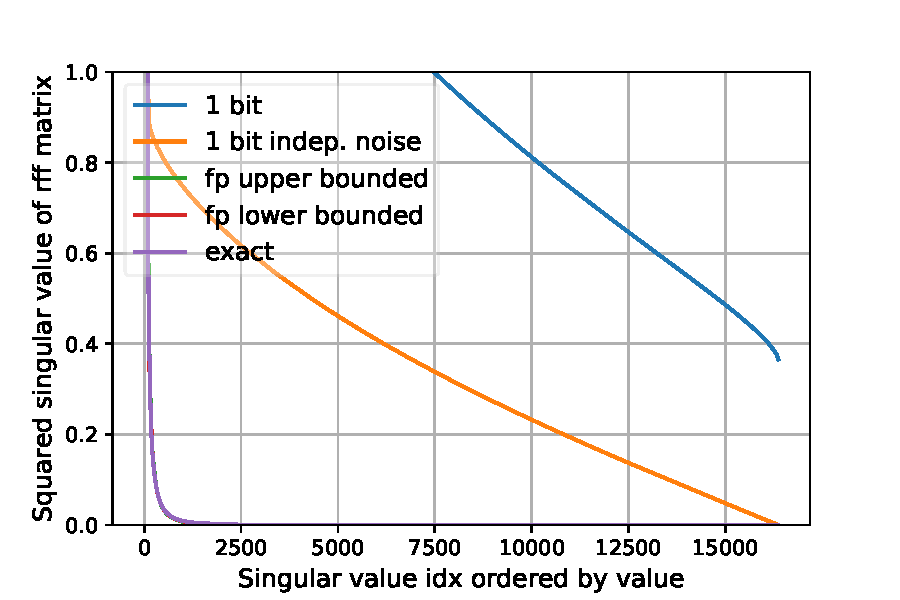
\includegraphics[width=.45\linewidth]{figures/different_spectrum_with_same_kernel_approx_error.pdf} \\
		(a) & (b)
	\end{tabular}
	\caption{Spectrum (eigen values) of the kernel matrix. (a) The spectrum from different precision representation under 3.2k bits memory budget (1024 full precision rffs) for the feature of each sample. (b) The spectrum from different precision representation under 25.6k bits memory budget (1024 full precision rffs) for the feature of each sample.}
\end{figure}


\begin{figure}
	\centering
	\begin{tabular}{c c}
		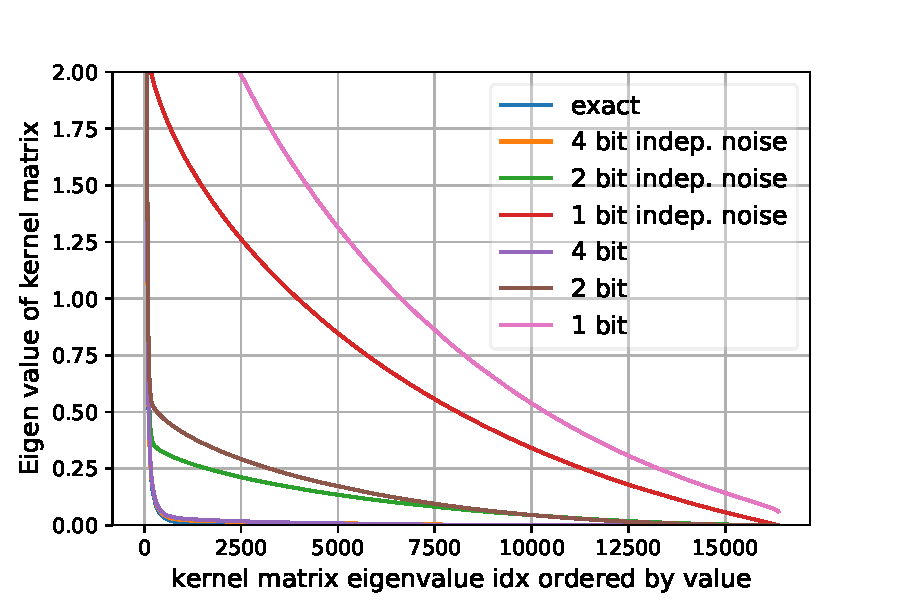
\includegraphics[width=.45\linewidth]{figures/spectrum_1024_indep.pdf} &
		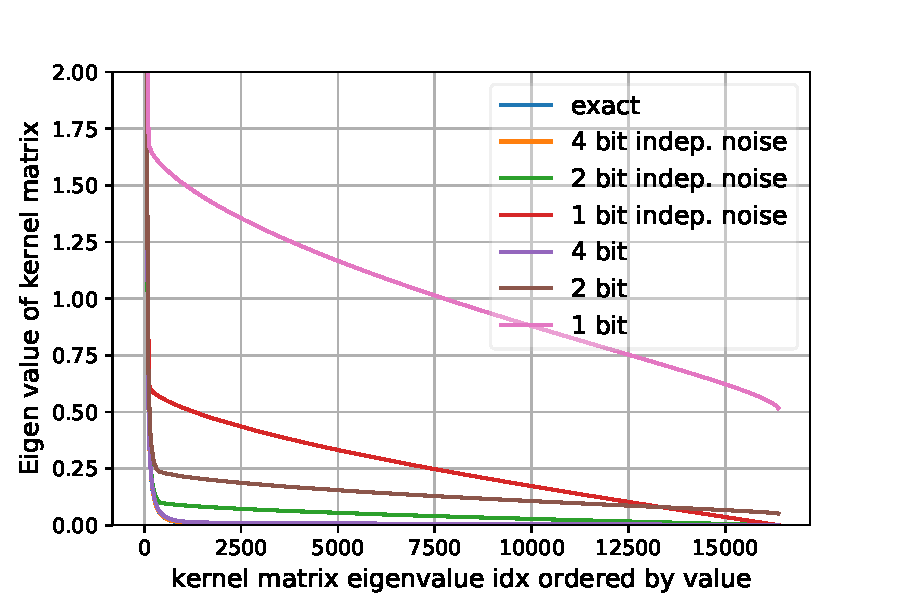
\includegraphics[width=.45\linewidth]{figures/spectrum_8192_indep.pdf} \\
		(a) & (b) \\
		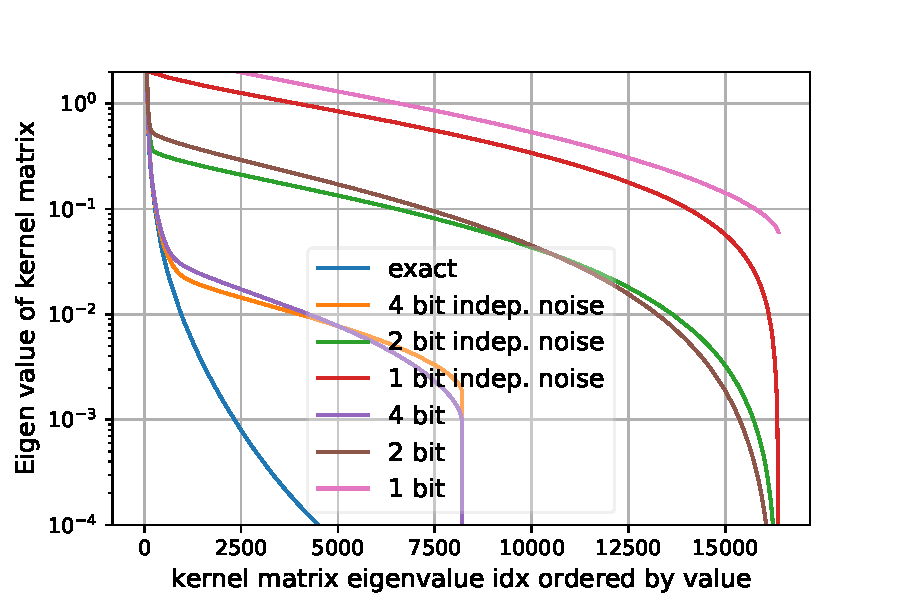
\includegraphics[width=.45\linewidth]{figures/spectrum_1024_indep_log.pdf} &
		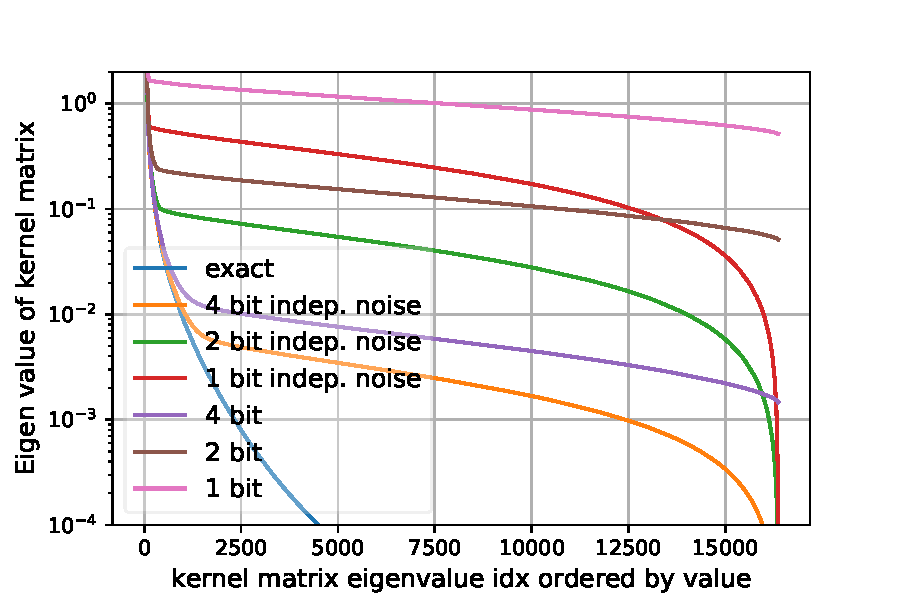
\includegraphics[width=.45\linewidth]{figures/spectrum_8192_indep_log.pdf} \\
		(c) & (d)
	\end{tabular}
	\caption{Spectrum (eigen values) of the kernel matrix. (a) The spectrum from different precision representation under 3.2k bits memory budget (1024 full precision rffs) for the feature of each sample. (b) The spectrum from different precision representation under 25.6k bits memory budget (1024 full precision rffs) for the feature of each sample.}
\end{figure}

%
%512 2 bits, 4096 fp 8192 fp, 4096 1 bit

